\section{Backlog Maintenance}

Managing Backlogs
\newline\newline
Backlogs can be easily maintained. Creating a backlog is the exact same process as creating any other type of model (via the File menu or the \'+\' button). Once you have opened the create window the only two things necessary for the creation of a backlog are the short name and the PO assigned to the backlog.
\newline
Adding a new story to a back log is easy. Simply select it from the story drop down (optionally give it a priority) and then press add. Prioritised stories will appear at the top of the table, ordered by their priority. Unprioritised stories will appear below them in alphabetical order. To remove a story simply click the X next to it.

\begin{figure}[H]
\centering
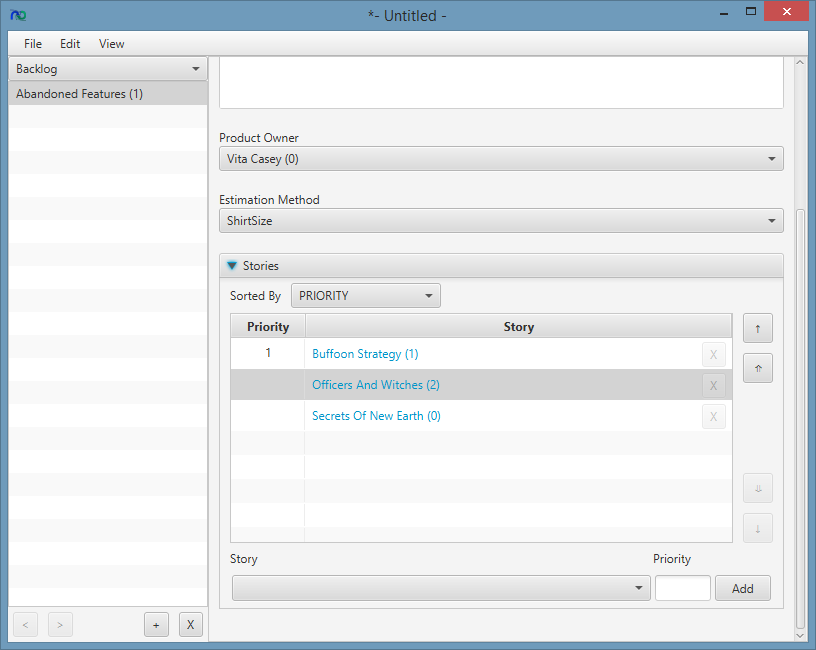
\includegraphics[width=\textwidth]{images/screenshots/backlogs.PNG}
\caption{The Backlogs Edit Pane}
\label{fig:new_project}
\end{figure}

\newline
To change the priority of a story simply select it and click on the up and down arrows to the side of the table; the small arrow buttons shift the story by one priority and the large up/down arrow buttons set the story's priority to one/unprioritised respectively. Alternatively, you may specify the exact priority you wish to change a story to by clicking in the priority column for the story you wish to move, the typing the new priority and pressing enter or else just clicking away.

\begin{figure}[H]
\centering
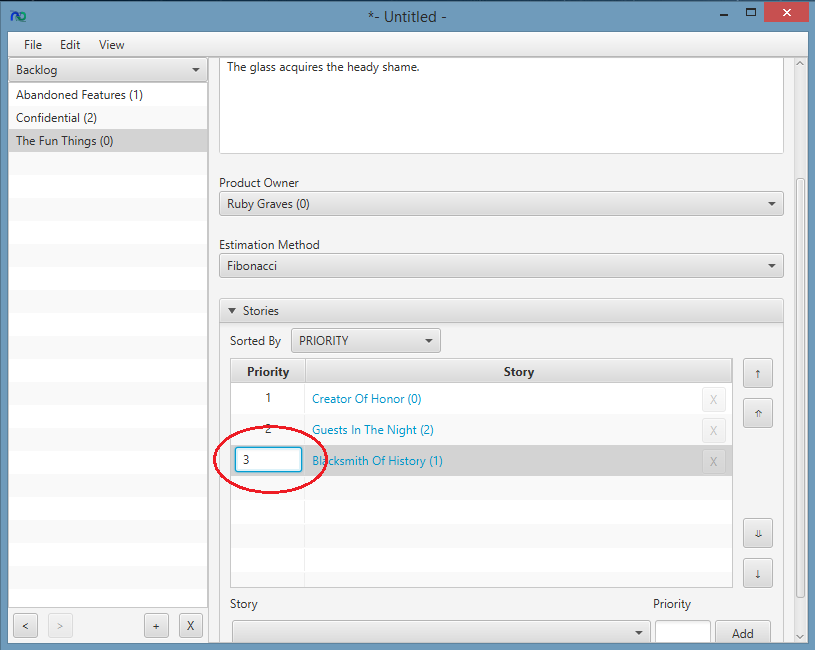
\includegraphics[width=\textwidth]{images/screenshots/editable_priority.PNG}
\caption{Editable Priorities}
\label{fig:new_project}
\end{figure}

\newline
If you wish to see a visual representation of the state of the backlog, you may selected the "highlight stories" item in the View menu. This will add a bar to the left of the table of stories that is coloured depending on the readiness state of the story it is beside. It is coloured red when the story depends on another story with a lower priority than itself, green when the story is ready and orange when it is almost ready but still requires an estimation.

\begin{figure}[H]
\centering
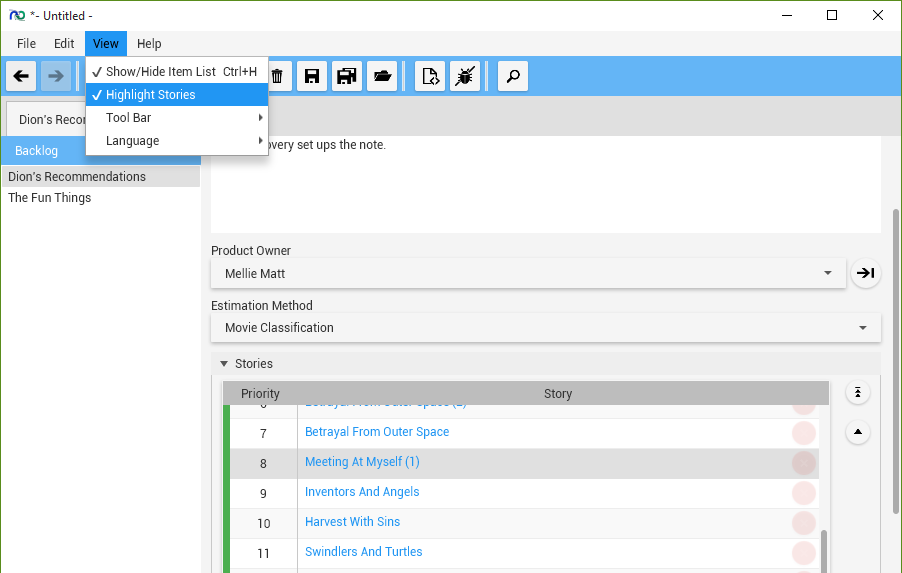
\includegraphics[width=\textwidth]{images/screenshots/story_highlighting.PNG}
\caption{Highlighting Stories}
\label{fig:new_project}
\end{figure}

\newline
Estimation Methods
\newline
Changing the estimation method changes how you estimate the difficulty of stories within the backlog. The supported types are Fibonacci (1,2,3,5,8,13), ShirtSizes (XS,S,M,L,XL,XXXL) and Movie Ratings (PG,G,M,R16,R18,Banned). You can change this at any time and the program will do its best to convert to the new scale.

\begin{figure}[H]
\centering
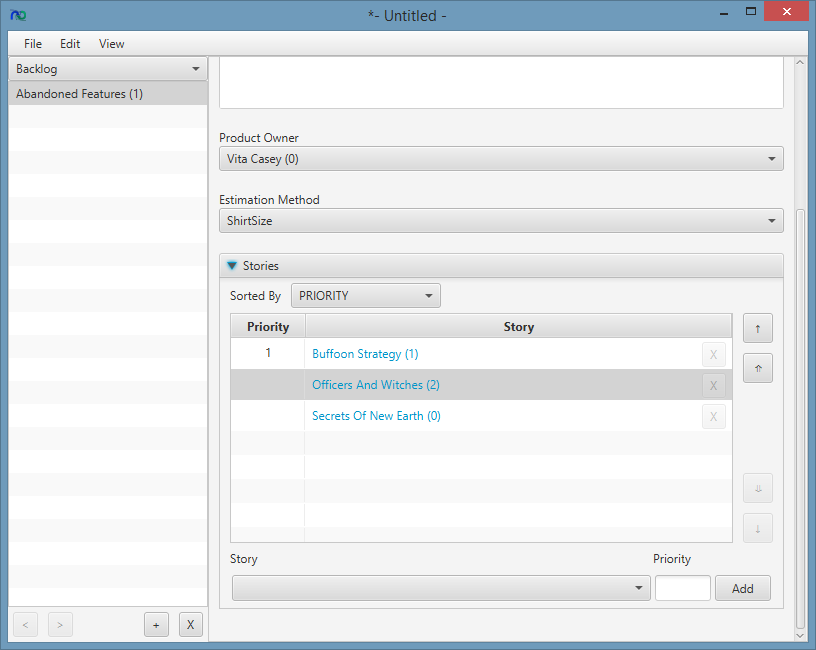
\includegraphics[width=\textwidth]{images/screenshots/backlogs.PNG}
\caption{The Estimate Method Choicebox}
\label{fig:new_project}
\end{figure}